%------------------ vorlage.tex ------------------------------------------------
%
%
%-------------------------------------------------------------------------------


%------------------ Präambel ---------------------------------------------------
\documentclass[envcountsame, envcountchap, deutsch, bibtotoc]{i-studis}
\usepackage{parskip} 
\usepackage[utf8]{inputenc}

\usepackage[a4paper]{geometry}
\usepackage[english, ngerman]{babel}
\usepackage{float}
\usepackage{nameref}

\usepackage[pdftex]{graphicx}
\usepackage{epstopdf}

\usepackage{listings}
\usepackage{makecell}

\usepackage[german, ruled, vlined]{algorithm2e}
\usepackage{amssymb, amsfonts, amstext, amsmath}
\usepackage{array}
%\usepackage[skip=10pt]{caption}
\usepackage[usenames, dvipsnames]{color}
\usepackage{xcolor}
%\usepackage{sectsty}
\usepackage{textcomp}
\usepackage{booktabs}
\usepackage{wrapfig}
\usepackage{titlesec}
\usepackage{blindtext}
\usepackage[shortcuts]{extdash}
% \usepackage{enumerate}
\usepackage{enumitem}

% Zitierpakete
\usepackage[style=apa,backend=biber,style=authoryear, maxcitenames=2]{biblatex}
% \DeclareLanguageMapping{german}{english}
\usepackage[pdftex, plainpages=false, breaklinks=true]{hyperref}
\usepackage[babel, german=quotes]{csquotes}
\addbibresource{Literatur.bib}

\usepackage{makeidx}
\usepackage{multicol}
\setlength{\tabcolsep}{0.5em}                  % for horizontal padding in tables

% Einstellungen für Code-Listings
\lstset{
        basicstyle=\ttfamily\scriptsize,       % print whole listing small and in monospace
        keywordstyle=\color{blue}\bfseries,    % underlined bold black keywords
        identifierstyle=,                      % nothing happens
        commentstyle=\color{red},              % white comments
        stringstyle=\ttfamily,                 % typewriter type for strings
        showstringspaces=false,                % no special string spaces
        framexleftmargin=7mm, 
        tabsize=3,
        showtabs=false,
        frame=single, 
        rulesepcolor=\color{blue},
        numbers=left,
        linewidth=146mm,
        xleftmargin=8mm,
        captionpos=b
}

\graphicspath{ {./Abbildungen/} }

\hypersetup{
    colorlinks,
    linkcolor={black},
    citecolor={blue!50!black},
    urlcolor={blue!80!black}
}

\makeindex

\pagestyle{myheadings}
\setlength{\textheight}{1.1\textheight}

%------------------ Titelseite -------------------------------------------------
\begin{document}
\setcounter{secnumdepth}{2}
\title{Analyse, Prognose und Visualisierung von New Yorker Taxifahrtdaten in einer Python-basierten, containerisierten Systemarchitektur}
\project{Seminararbeit - Advanced Analytics}
% \degree{Bachelor of Science (B.Sc.)}                    % Nur bei Abschlussarbeit!
\address{im Studiengang Wirtschaftsinformatik an der\\Hochschule Trier}

\author{Paul Jakob}
\supervisorFirst{Prof. Dr. Martin Vogt}
\matrikelnummer{982.131}
\fachbereich{Wirtschaft}
\studiengang{Wirtschaftsinformatik}
\submitdate{11.06.2026}

\mytitlepage

%------------------ Vorwort, Kurzfassung, Verzeichnisse ------------------------
\frontmatter
\tableofcontents						%Inhaltsverzeichnis
\listoffigures                        %Abbildungsverzeichnis
\listoftables                           %Tabellenverzeichnis
%------------------ Kapitel ----------------------------------------------------
\mainmatter
\chapter{Einleitung}
\sloppy
Die Fähigkeit von IT-Infrastrukturen, sich dynamisch an variierende Anforderungen anzupassen, ist eine zentrale Anforderung zeitgemäßer Softwarearchitektur (vgl. Bharadwaj et al. 2013, S. 471 f.). Unternehmerische Agilität, verstanden als die Kapazität einer Organisation, schnell und effektiv auf technische wie fachliche Veränderungen zu reagieren, setzt voraus, dass Systeme bedarfsgerecht skaliert werden können, ohne dauerhaft physische Ressourcen binden zu müssen (vgl. Tallon/Pinsonneault 2011, S. 463 f.). Gleichzeitig gewinnt die digitale Souveränität an Bedeutung, die den selbstbestimmten Umgang einer Organisation mit ihren Infrastrukturentscheidungen, Daten und Technologieabhängigkeiten bezeichnet (vgl. Couture/Toupin 2019, S. 2 ff.). Während klassische Systeme oft starre Strukturen aufweisen, erfordern Big-Data-Szenarien heuzutage Architekturen, die Souverinität und Agilität inhärent abbilden (vgl. Marz/Warren 2015, S. 4 ff.).

Als empirische Grundlage dient der NYC Taxi Trip Data-Datensatz, der umfangreiche Informationen zu Taxifahrten in New York City enthält. Anhand dieses Datensatzes werden Datenoperationen von der Berechnung deskriptiver Kennzahlen über explorative Visualisierungen bis hin zum Training von Vorhersagemodellen durchgeführt, um die Leistungsfähigkeit der Python-basierten, containerisierten Systemarchitektur unter realitätsnahen Lastbedingungen zu demonstrieren. Im Vordergrund stehen dabei nicht die domänenspezifischen Erkenntnisse aus den Verkehrsdaten selbst, sondern die systemarchitektonischen Herausforderungen, eine robuste und zugleich flexible Umgebung für Softwareentwicklung und Betrieb zu schaffen. Der Einsatz von Docker-Containern gewährleistet dabei Portabilität, elastische Skalierbarkeit und nahtlose Plattformunabhängigkeit (vgl. Merkel 2014, S. 2 ff.).

Ziel dieser Arbeit ist die Konzeption und prototypische Implementierung einer modularisierten Infrastruktur, die durch konsequente Diensttrennung und Orchestrierung eine skalierbare Datenverarbeitungspipeline realisiert, vom Datenimport über die Aufbereitung bis zur Bereitstellung via API sowie der finalen Visualisierung und Vorhersage (vgl. Newman 2015, S. 1 ff.).
\chapter{Konzeptionelle Grundlagen}
\section{Technische Grundlagen}
\subsection{Containerarchitektur}
Containerisierung bezeichnet die Kapselung von Anwendungen samt ihrer Laufzeitabhängigkeiten in isolierte, portable Einheiten – sogenannte Container. Im Unterschied zu klassischen virtuellen Maschinen teilen sich Container den Kernel des Host-Betriebssystems, was einen erheblich geringeren Ressourcenoverhead sowie kürzere Startzeiten bedingt (vgl. Merkel 2014, S. 2 f.). Docker hat sich als De-facto-Standard für die Erstellung und den Betrieb von Containern etabliert, indem Laufzeitumgebungen durch deklarative Dockerfiles vollständig reproduzierbar definiert werden (vgl. Anderson 2015, S. 1 f.).

Für Multi-Container-Anwendungen erweitert Docker Compose diesen Ansatz um eine zentrale, deklarative Konfigurationsdatei zur Vernetzung und Steuerung mehrerer Dienste (vgl. Stoneman 2020, S. 14 ff.). In Verbindung mit dem Microservice-Paradigma – bei dem funktionale Einheiten in lose gekoppelte, unabhängig deploybare Dienste zerlegt werden – entfaltet Containerisierung ihr volles Potenzial: Einzelne Komponenten lassen sich bedarfsgerecht skalieren, unabhängig aktualisieren und replizieren, ohne das Gesamtsystem zu beeinträchtigen (vgl. Newman 2015, S. 1 ff.).

\subsection{Anwendung von Python}
Python bildet aufgrund seiner lesbaren Syntax und seines umfangreichen Bibliotheksökosystems die technologische Basis der vorliegenden Systemarchitektur (vgl. VanderPlas 2016, S. 2 f.). Die Datenverarbeitung stützt sich auf pandas, dessen DataFrame-Konzept tabellarische Daten effizient vorhält und für Einlesen, Bereinigung sowie Aggregation der Rohdaten eingesetzt wird (vgl. McKinney 2017, S. 97 ff.). Das spaltenorientierte Apache-Parquet-Format wird über PyArrow eingebunden und bietet signifikante Lese- und Speichervorteile gegenüber zeilenorientierten Formaten wie CSV (vgl. Vohra 2016, S. 11 f.). Für die Imputation fehlender Werte kommt der IterativeImputer aus scikit-learn zum Einsatz, der das MICE-Verfahren implementiert (vgl. Pedregosa et al. 2011, S. 2825 f.).

Die statistische Modellierung stützt sich auf statsmodels, das Generalisierte Lineare Modelle (GLM) und Kleinstquadrateschätzung (OLS) über eine patsy-basierte Formelschnittstelle bereitstellt (vgl. Seabold/Perktold 2010, S. 93). Die HTTP-Schnittstellen zwischen den Containerdiensten werden über Flask in Kombination mit dem WSGI-Server Waitress realisiert (vgl. Grinberg 2018, S. 4 ff.). Die Visualisierungsschicht basiert auf Streamlit und Plotly Express, die interaktive Webanwendungen in reinem Python ermöglichen (vgl. Tamminga 2022, S. 1 f.).

\subsection{REST-API}
Representational State Transfer (REST) bezeichnet einen von Roy Thomas Fielding formalisierten Architekturstil für netzwerkbasierte Softwareschnittstellen, der auf dem HTTP-Protokoll aufsetzt (vgl. Fielding 2000, S. 76 ff.). Kernprinzipien sind strikte Client-Server-Trennung, Zustandslosigkeit sowie ein einheitliches Interface: Ressourcen werden über stabile URIs adressiert und über standardisierte HTTP-Methoden manipuliert, wobei Antworten typischerweise im JSON-Format übermittelt werden (vgl. Richardson/Ruby 2007, S. 7 ff.). Im Kontext von Microservice-Architekturen fungieren REST-APIs als primärer Kommunikationskanal zwischen Diensten und gewährleisten so funktionale Isolation sowie horizontale Skalierbarkeit (vgl. Newman 2015, S. 1 ff.).

\section{Vorstellung des Datensatzes}
Die empirische Grundlage dieser Arbeit bildet das Open-Data-Repertoire der New York City Taxi \& Limousine Commission (TLC). Der Datensatz umfasst detaillierte Aufzeichnungen über Millionen von Individualverkehrsbewegungen im Stadtgebiet New Yorks und gilt aufgrund seiner hohen zeitlichen sowie räumlichen Auflösung als Standardreferenz in der raumzeitlichen Datenanalyse. Herangezogen wird primär das Segment der „Yellow Taxi Data", welches den regulären Taxibetrieb im Stadtzentrum abbildet.

Strukturell handelt es sich um hochgradig granulare Transaktionsdaten: Jeder Datensatz repräsentiert eine einzelne Beförderung und beinhaltet Zeitstempel für Aufnahme und Absetzen der Fahrgäste, geographische Taxizonen sowie die zurückgelegte Fahrtstrecke. Ergänzend sind Tarifstrukturen (Fahrpreis, Steuern, Zuschläge) und die gewählte Zahlungsart erfasst. Angesichts eines Volumens von mehreren Gigabyte pro Jahr erfüllt der Datensatz die Charakteristika von Big Data. Die Vorverarbeitung erfordert dabei eine systematische Behandlung von Ausreißern – etwa unplausible Fahrtdauern oder fehlerhafte Tarifangaben – sowie vereinzelter Inkonsistenzen. Durch die Kombination aus zeitlicher Dichte und geographischer Präzision lassen sich komplexe urbane Mobilitätsmuster extrahieren, Nachfragespitzen identifizieren und ökonomische Trends ableiten.

\section{Angewendete Methoden}
\subsection{Multiple Imputation}
Fehlende Werte stellen in empirischen Datensätzen ein systematisches Problem dar, das bei naiver Behandlung zu verzerrten Schätzungen und einem Verlust statistischer Effizienz führt. Der listenweise Ausschluss unvollständiger Beobachtungen setzt voraus, dass Daten vollständig zufällig fehlen (MCAR, Missing Completely at Random) – eine Annahme, die in der Praxis selten zutrifft (vgl. Little/Rubin 2002, S. 41 ff.).

Als methodisch überlegene Alternative erzeugt die Multiple Imputation mehrere plausible Datensätze, die jeweils unterschiedliche Imputationswerte enthalten und damit die Unsicherheit über den wahren, nicht beobachteten Wert explizit abbilden (vgl. Rubin 1987, S. 75 ff.). Die leistungsfähige Ausprägung MICE (Multiple Imputation by Chained Equations) spezifiziert für jede unvollständige Variable ein separates Regressionsmodell und durchläuft diese Kette konditionaler Modelle iterativ bis zur Konvergenz (vgl. van Buuren/Groothuis-Oudshoorn 2011, S. 7 ff.). In scikit-learn ist dieses Prinzip als IterativeImputer implementiert (vgl. Pedregosa et al. 2011, S. 2826).

\subsection{Generalisiertes Lineares Modell}
Die klassische lineare Regression setzt eine kontinuierliche, normalverteilte Zielvariable voraus. Für Zähldaten oder strikt positive Mengengrößen sind diese Annahmen verletzt, was zu ineffizienten Schätzern führt (vgl. McCullagh/Nelder 1989, S. 1 ff.). Das von Nelder und Wedderburn 1972 eingeführte Generalisierte Lineare Modell (GLM) überwindet diese Einschränkungen durch drei Komponenten: einen linearen Prädiktor, eine Verknüpfungsfunktion sowie eine Verteilungsannahme aus der Exponentialfamilie (vgl. Nelder/Wedderburn 1972, S. 370 ff.). Für Zähldaten eignet sich die Poisson-Verteilung; bei Überdispersion bietet die Negativ-Binomialverteilung eine robustere Alternative (vgl. Cameron/Trivedi 2013, S. 75 f.). Für strikt positive, stetige Zielgrößen stehen Gamma- sowie Invers-Gaußsche Verteilung zur Verfügung (vgl. McCullagh/Nelder 1989, S. 292 ff.). Die Parameterschätzung erfolgt über die Maximum-Likelihood-Methode; zur Modellbewertung dienen das Akaike-Informationskriterium (AIC) sowie die p-Werte der Koeffizientenschätzungen (vgl. Fahrmeir/Tutz 2001, S. 86 ff.).

\chapter{Hauptteil}

\section{Technische Architektur}

\begin{figure}[htb]
    \centering
    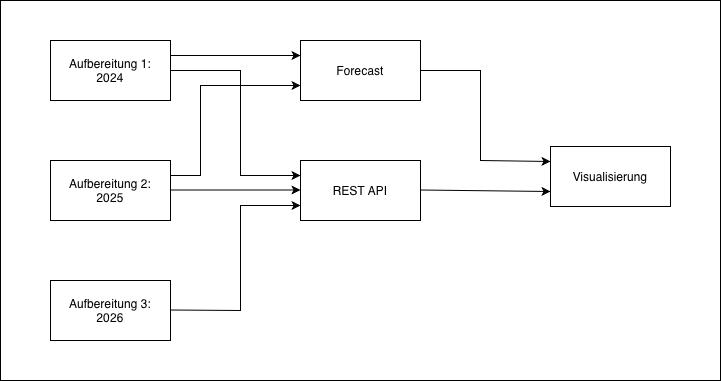
\includegraphics[width=\textwidth]{Abbildungen/Containerarchitektur.png}
    \caption[Containerarchitektur]{Containerarchitektur\footnotemark}
    \label{fig:containerarchitektur}
\end{figure}
\footnotetext{Eigene Darstellung.}

Die realisierte Systemarchitektur setzt sich aus sechs funktional getrennten Docker-Containern zusammen, die über ein gemeinsames Bridge-Netzwerk miteinander kommunizieren (vgl. Abbildung \ref{fig:containerarchitektur}). Das Fundament bilden drei identische Instanzen des Aufbereitungsdienstes (\texttt{aa\_aufbereitung\_1} bis \texttt{aa\_aufbereitung\_3}), die durch containerindividuelle Volume-Mounts jeweils spezifische Datenzeiträume verarbeiten: die Perioden 2025 sowie Januar 2026. Die mehrfache Instanziierung desselben Container-Images demonstriert das Kernprinzip horizontaler Skalierbarkeit – eine einmal definierte Laufzeitumgebung kann ohne Anpassung des Anwendungscodes für unterschiedliche Eingabedaten repliziert werden (vgl. Merkel 2014, S.~4~f.). Jede Instanz exponiert eine REST-konforma HTTP-Schnittstelle auf Port 8080 und stellt aufbereitete Datensätze sowie Spalteninformationen für nachgelagerte Dienste bereit. Um eine kontrollierte Startreihenfolge zu gewährleisten, definiert \texttt{docker-compose.yaml} Gesundheitsprüfungen auf Basis von HTTP-Anfragen sowie \texttt{depends\_on}-Bedingungen, die sicherstellen, dass kein nachgelagerter Dienst startet, bevor alle Aufbereitungsinstanzen betriebsbereit sind (vgl. Stoneman 2020, S.~14~ff.).

Der Forecast-Container (\texttt{aa\_forecast}) bezieht die aufbereiteten Rohdaten über konfigurierbare HTTP-Verbindungen aus allen drei Aufbereitungsinstanzen, führt sie zu einem gemeinsamen DataFrame zusammen und stellt darauf basierend statistische Vorhersagemodelle über eine eigene REST-API auf Port 9000 bereit. Der API-Container (\texttt{aa\_api}) hingegen aggregiert die historischen Daten ausschließlich nach zeitlichen Dimensionen und dient als stabiler Datenzugangspunkt für die Visualisierungsschicht. Den Abschluss des Datenflusses bildet der Visualisierungs-Container (\texttt{aa\_visual}), der eine interaktive Webanwendung auf Basis von Streamlit bereitstellt und sowohl historische als auch prognostizierte Kennzahlen grafisch aufbereitet. Die konsequente Diensttrennung entspricht dem Microservice-Paradigma, das funktionale Einheiten in lose gekoppelte, unabhängig deploybare Dienste zerlegt und so eine gezielte Skalierung einzelner Komponenten ohne Beeinträchtigung des Gesamtsystems ermöglicht (vgl. Newman 2015, S.~1~ff.).

\section{Aufbereitung der Daten}

Die Datenaufbereitung gliedert sich in drei aufeinanderfolgende Phasen: den Datenimport, die Bereinigung sowie die Merkmalsgenerierung. Der Import unterstützt sowohl das CSV- als auch das spaltenorientierte Apache-Parquet-Format, wobei Parquet-Dateien blockweise über PyArrow eingelesen werden, um den Hauptspeicherverbrauch zu kontrollieren (vgl. Vohra 2016, S.~11~f.). CSV-Dateien werden mittels \texttt{pandas} in Chunks von 100.000~Zeilen verarbeitet; im Testbetrieb wird über zufälliges Zeilen-Sampling der Datensatz auf einen repräsentativen Bruchteil reduziert, um Entwicklungszyklen zu beschleunigen. Sämtliche Zeitstempelfelder (\texttt{tpep\_pickup\_datetime}, \texttt{tpep\_dropoff\_datetime}) werden in ein einheitliches Zeichenkettenformat überführt, aus dem Jahr, Monat, Tag und Stunde als separate numerische Spalten extrahiert werden (vgl. McKinney 2017, S.~97~ff.).

Die Bereinigungsroutine entfernt systematisch unplausible Datensätze: Fahrten mit einem Fahrpreis von null oder negativen Werten werden ausgeschlossen, ebenso Fahrtstrecken außerhalb des Intervalls $(0, 100]$~Meilen sowie Passagierzahlen kleiner eins oder größer sechs. Extremwerte des Fahrpreises oberhalb des 99,5.~Perzentils werden gekappt, um den Einfluss vereinzelter Datenerfassungsfehler auf nachgelagerte Modelle zu begrenzen.

Die Merkmalsgenerierung überführt die Rohdaten in ein für statistische Modellierung geeignetes Format. Aus dem Abholzeitpunkt werden Wochentag, Wochenendindikator, Jahreszeit sowie binäre Variablen für Feiertage (auf Basis der US-amerikanischen gesetzlichen Feiertage), den Tag vor und nach einem Feiertag sowie die Rush-Hour-Perioden (7–9~Uhr und 16–18~Uhr) abgeleitet. Zur Abbildung der inhärenten Zyklizität zeitlicher Dimensionen werden Wochentag und Monat mittels trigonometrischer Transformation in Sinus- und Kosinuskomponenten überführt:

\begin{equation}
    x_{\sin} = \sin\!\left(\frac{2\pi \cdot t}{T}\right), \quad x_{\cos} = \cos\!\left(\frac{2\pi \cdot t}{T}\right)
\end{equation}

Dabei bezeichnet $t$ den diskreten Zeitindex (Wochentag $0$–$6$ bzw. Monat $1$–$12$) und $T$ die Periodenlänge. Diese Kodierung stellt sicher, dass die Distanz zwischen Montag und Sonntag im Merkmalsraum der intuitiven zyklischen Nähe entspricht – eine Eigenschaft, die lineare Merkmale nicht abbilden können (vgl. Fahrmeir/Tutz 2001, S.~10~f.).

Für Fahrten mit Barzahlung (\texttt{payment\_type}~=~2) weist der Datensatz strukturell fehlende Trinkgeldwerte auf, da Trinkgelder bei dieser Zahlungsart nicht elektronisch erfasst werden. Zur Imputation wird das MICE-Verfahren (\textit{Multiple Imputation by Chained Equations}) eingesetzt, das für jede unvollständige Variable ein separates Regressionsmodell spezifiziert und diese Kette konditionaler Modelle iterativ bis zur Konvergenz durchläuft (vgl. van Buuren/Groothuis-Oudshoorn 2011, S.~7~ff.). Die Scikit-learn-Implementierung \texttt{IterativeImputer} verwendet als Prädiktoren Gesamtbetrag, Fahrpreis und Fahrtdistanz; negative Imputationswerte werden anschließend auf null begrenzt, da Trinkgelder definitionsgemäß nicht negativ sein können (vgl. Pedregosa et~al. 2011, S.~2826). Durch dieses Vorgehen wird auf den listenweisen Ausschluss von Barzahlungsfahrten verzichtet, was die Stichprobengröße erhält und potenzielle Verzerrungen durch systematisch fehlende Werte reduziert (vgl. Little/Rubin 2002, S.~41~ff.).

Die aufbereiteten Daten werden als vollständiger JSON-kodierter DataFrame über den \texttt{/miced\_data}-Endpunkt der jeweiligen Aufbereitungsinstanz bereitgestellt; die Spaltenliste ist separat über \texttt{/columns} abrufbar und wird beim Start nachgelagerter Dienste zur Kompatibilitätsprüfung herangezogen.

\section{Modellierung und Prognose}

Der Forecast-Dienst realisiert eine anfrage-gesteuerte statistische Modellierung: Für jede eingehende HTTP-Anfrage werden Aggregationsmethode, Gruppierungsdimensionen und Zielvariable aus den URL-Parametern extrahiert, ein Modell auf den entsprechend aggregierten Trainingsdaten angepasst und Vorhersagen für den Zielzeitraum 2026 generiert.

\subsection{Merkmalsauswahl und Aggregation}

Abhängig vom angefragten Zeitgranular werden unterschiedliche Merkmalssätze aktiviert: Für tagesgenaue Anfragen fließen zyklische Wochentag-Kodierungen sowie alle binären Tagesmerkmale (Wochenende, Feiertag, Rush-Hour etc.) in die Modellformel ein; für monatliche Anfragen werden die trigonometrischen Monatskodierungen hinzugefügt. Werden stündliche Dimensionen wie \texttt{pickup\_hour} einbezogen, ergänzt der Dienst automatisch den Rush-Hour-Indikator. Die Zielvariable und alle kategorialen Prädiktoren werden über eine \texttt{patsy}-Formel spezifiziert, wobei kategoriale Variablen automatisch als Dummy-Variablen kodiert werden. Für Vorhersagen wird ein kartesisches Produkt aller zulässigen Merkmalsausprägungen als Prädiktionsrahmen aufgespannt, sodass vollständige Vorhersagegitter entstehen.

\subsection{Modellauswahl und Schätzung}

Je nach Aggregationsmethode der Zielvariablen werden unterschiedliche Modellklassen eingesetzt. Bei Zählaggregationen (\texttt{count}) werden ein Poisson-GLM sowie – zur Behandlung von Überdispersion – ein Negativ-Binomial-GLM angepasst (vgl. Cameron/Trivedi 2013, S.~75~f.). Bei stetigen Zielgrößen (\texttt{mean}) stehen neben dem Gauß-GLM, sofern die Zielvariable strikt positiv ist, zusätzlich ein Gamma- sowie ein Invers-Gauß-GLM zur Verfügung, die asymmetrisch verteilte, rechtsschiefe Größen wie Fahrpreise adäquater modellieren (vgl. McCullagh/Nelder 1989, S.~292~ff.). Ergänzend wird stets ein OLS-Modell (\textit{Ordinary Least Squares}) als Referenzmodell geschätzt. Alle GLM-Parameter werden über Maximum-Likelihood-Schätzung bestimmt (vgl. Nelder/Wedderburn 1972, S.~370~ff.); die Implementierung erfolgt über \texttt{statsmodels} mit patsy-basierter Formelschnittstelle (vgl. Seabold/Perktold 2010, S.~93).

Für stetige Zielgrößen wird vor der Modellanpassung eine logarithmische Transformation der Zielvariablen mittels $\log(1 + y)$ vorgenommen. Diese Varianzstabilisierung begegnet der typischen rechtsschieven Verteilung von Betragsgrößen und verbessert die Anpassungsgüte linearer Prädiktoren; die Rücktransformation der Vorhersagen erfolgt über $\exp(\hat{y}) - 1$ (vgl. Fahrmeir/Tutz 2001, S.~18~f.).

Zur Modellbewertung liefert der Dienst neben den eigentlichen Vorhersagen eine Zusammenfassung aller angepassten Modelle, die Koeffizientenschätzungen, zugehörige $p$-Werte, das Akaike-Informationskriterium (AIC) sowie – für das OLS-Modell – das Bestimmtheitsmaß $R^2$ und dessen adjustierte Variante enthält. Das AIC erlaubt einen modellklassenübergreifenden Vergleich unter Berücksichtigung der Modellkomplexität: Ein niedrigerer AIC-Wert indiziert ein günstigeres Verhältnis zwischen Anpassungsgüte und Parameterzahl (vgl. Fahrmeir/Tutz 2001, S.~86~ff.). Die Modellzusammenfassung wird über die API an die Visualisierungsschicht übermittelt und dort tabellarisch nach AIC sortiert dargestellt, sodass Nutzer das leistungsfähigste Modell für den jeweiligen Anwendungsfall identifizieren können.

\section{Visualisierung}

Die Visualisierungsschicht ist als interaktive Webanwendung in Streamlit realisiert und bindet sowohl den historischen API-Dienst als auch den Forecast-Dienst als konfigurierbare Datenquellen ein (vgl. Tamminga 2022, S.~1~f.). Die Seitenleiste erlaubt die kontextadaptive Auswahl von Zeiträumen, Kennzahlen, Aggregationsmethoden und Gruppierungsdimensionen; verfügbare Zeiträume werden dabei dynamisch aus dem \texttt{/data\_summary}-Endpunkt der verbundenen APIs bezogen, sodass die Oberfläche stets nur tatsächlich vorhandene Daten anbietet.

Für die Ergebnisdarstellung stehen fünf Diagrammtypen zur Verfügung: Liniendiagramme für zeitliche Verläufe, Balkendiagramme für ein- und zweidimensionale Vergleiche, Heatmaps zur Darstellung zweidimensionaler Kreuztabellen, Streudiagramme sowie dreidimensionale Streudiagramme für mehrdimensionale Beziehungen. Alle Diagramme werden mit Plotly Express gerendert und sind interaktiv zoom- und filterbar (vgl. Tamminga 2022, S.~1~f.). Oberhalb jeder Visualisierung werden drei Kennzahlen – Summe, Durchschnitt und Datensatzanzahl – als kompakte Metriken hervorgehoben.

Die Anfragestrategie passt sich automatisch an den ausgewählten Zeitgranular an: Bei tagesgenauen Anfragen wird für jeden selektierten Tag eine separate API-Anfrage gestellt und die Ergebnisse anschließend zusammengeführt; bei monatlichen oder jährlichen Anfragen wird entsprechend auf Monats- bzw. Jahresebene aggregiert. Sind sowohl der historische als auch der Forecast-Dienst aktiv, werden Prognose- und Ist-Daten für identische Zeitperioden kombiniert, wobei Duplikate durch Priorisierung des historischen Dienstes aufgelöst werden. Kategoriale Variablen wie Zahlungsart, Anbieter und Tarifcode werden clientseitig auf lesbare Bezeichnungen abgebildet. Über dynamische Filterpanels können Nutzer die dargestellten Merkmalskombinationen interaktiv einschränken; der vollständige Datensatz ist zudem als CSV-Datei exportierbar.

\section{Mögliche Analysen}

Das realisierte System ermöglicht eine Vielzahl deskriptiver und prädiktiver Analysen. Deskriptiv lassen sich Nachfrageschwankungen über Tagesstunden, Wochentage und Monate verfolgen und mit Feiertagen oder Rush-Hour-Perioden in Beziehung setzen. Die Gruppierung nach Zahlungsart erlaubt Rückschlüsse auf Kundenpräferenzen; eine Kreuzauswertung von Anbieter und Tarifzone gibt Hinweise auf räumliche Nachfragekonzentrationen. Durch Gegenüberstellung der imputierten Trinkgelddaten mit Fahrpreisen und Zahlungsarten lassen sich Einflussfaktoren auf das Trinkgeldverhalten explorieren.

Prädiktiv kann das System Zielgrößen wie Fahrtenanzahl, durchschnittlicher Fahrpreis oder Trinkgeldhöhe für beliebige Kombinationen aus Tageszeit, Wochentag und Saisonmerkmalen im Prognosezeitraum 2026 schätzen. Der modellübergreifende Vergleich über das AIC ermöglicht dabei eine datengetriebene Auswahl des geeignetsten Modells je Anwendungsfall. Die Integration von Prognosedaten und historischen Daten in einer gemeinsamen Visualisierung erlaubt schließlich eine unmittelbare visuelle Validierung der Modellgüte.
\chapter{Schlussbetrachtung}
Diese Bachelor-Thesis hatte zum Ziel, ... Dazu wurden... Es kann festgehalten werden, dass...
...
Die Vorstellungen von Professorinnen und Professoren können sich bezüglich der formalen Ausgestaltungen leicht unterscheiden (z.\,B. in puncto anzuwendender Zitierform, Schriftarten, Größe der Seitenränder etc.). Es empfiehlt sich daher immer, die gewünschten Formatvorgaben mit dem jeweiligen Betreuer vorab kurz abzusprechen.

%------------------ Literaturverzeichnis & Index -------------------------------
\backmatter
\printbibliography
\printindex												% Index (optional)
%------------------ Anhänge ----------------------------------------------------
\begin{appendix}
	%\chapter{Glossar}

\abbreviation{$\text{BK}_{i,t}$}    {Börsenkurs der Aktie $i$ zum Zeitpunkt $t$}
\abbreviation{$\text{D}_{i,t}$}	    {Dividendenzahlung der Aktie $i$ zum Zeitpunkt $t$}
\abbreviation{$\text{r}_i$}         {Rendite der Aktie $i$}
\abbreviation{...}      		    {...}

						% Glossar (optional)
    %\chapter{Häufige Fehler in Seminar- und Abschlussarbeiten}
An dieser Stelle wird ein Überblick darüber gegeben, welche Fehler in schriftlichen wissenschaftlichen Arbeiten häufig auftreten. Die genannten Punkte können zur Reflektion und zur Prüfung in allen Phasen des Verfassens einer Seminar- oder Abschlussarbeit herangezogen werden. 

\section{Inhalt}

\emph{Erfassung der Aufgabenstellung}
\begin{itemize}
    \item Das Thema wird nicht vollständig erfasst, einzelne Themenbestandteile werden nicht berücksichtigt, die Beziehungen zwischen den Themenbestandteilen werden nicht herausgearbeitet. 
    \item Es wird ein Thema bearbeitet, welches sich nicht aus der Aufgabenstellung erschließt.
\end{itemize}

\emph{Aufbau der Arbeit und Inhalt}
\begin{itemize}
    \item Technische Gliederungsfehler
    \item Der Fluss der Gliederung ist nicht ersichtlich.
    \item Die Gliederungsteile bauen nicht aufeinander auf, sie stehen vielmehr isoliert nebeneinander.
    \item Die Überschriften sind nicht aussagekräftig.
    \item Eine Überschrift deckt sich vollständig mit dem Thema der Arbeit.
\end{itemize}

\emph{Anmerkungen zum Inhalt}
\begin{itemize}
    \item Problemstellung und Zielsetzung der Arbeit werden nur oberflächlich angerissen.
    \item Allgemeinplätze: „Globalisierung und zunehmende Dynamik ...“
\end{itemize}

\newpage
\emph{Eigenständigkeit der erbrachten Leistung}
\begin{itemize}
    \item Mangelnde Eigenständigkeit der erbrachten Leistung
    \item Zu viele direkte Zitate, mangelnde Reflektion in eigenen Worten
    \item Abbildungen und Tabellen werden 1:1 übernommen ohne kontextbezogene Eigenleistung und Darstellung. 
\end{itemize}


    %\chapter{Wissenschaftliche Methode}

\emph{Begriffsbildung, Definition, Abgrenzung}
\begin{itemize}
    \item Begriffe werden nicht eingeführt, gar nicht oder aber erst später definiert.
    \item Falsche oder ungenaue Begriffsbildungen und -verwendungen
    \item Begriffe werden nicht überschneidungsfrei voneinander abgegrenzt.
    \item Gleiche Tatbestände werden mit unterschiedlichen Begriffen belegt.
    \item Mit der verwendeten Quelle wechselt die Notation, d. h. Begriffe werden mit unterschiedlichen Symbolen belegt.
\end{itemize}

\emph{Gedankenführung und Aufbau}
\begin{itemize}
    \item Die Kapitelüberschriften behandeln nicht oder nicht exakt das Thema der Arbeit.
    \item Sämtliche Überschriften einer tieferen Gliederungsebene behandeln nicht oder nicht exakt das Thema der Überschrift auf der nächst höheren Gliederungsebene.
    \item Es erfolgt die Untergliederung eines Absatzes, wobei nur ein Unterpunkt ausgewiesen wird: z. B. Absatz 3 soll untergliedert werden. Es wird nur ein Absatz 3.1 aufgeführt, 3.2, 3.3 usw. fehlen.
    \item Die Ausführungen innerhalb eines Absatzes betreffen nicht die Überschrift des Absatzes.
\item Der Fluss der Gedanken muss auf jeder Ebene deutlich sein; dies gilt sowohl für die gesamte Gliederung als auch für einzelne Absätze (auch die müssen strukturiert sein und einem „roten Faden“ folgen).
    \item Oft fehlen die Überleitungen zwischen einzelnen Kapiteln, der Gang der Arbeit wird nicht inhaltlich begründet (sowohl in der Einleitung als auch in den folgenden Ausführungen).
\end{itemize}

\newpage
\emph{Ergebnisbildung}
\begin{itemize}
    \item Angesichts einer in der Einleitung beschriebenen Problemstellung fehlt ein Diskussionsergebnis bzw. es ist unklar.
    \item Das Ergebnis hat wenig mit der in der Einleitung aufgeworfenen Problemstellung sowie den Untersuchungszielen zu tun.
    \item Das Ergebnis wird nicht eindeutig formuliert, der Kandidat „drückt“ sich um eine Stellungnahme.
\end{itemize}
\end{appendix}
\end{document}